\addtocontents{toc}{\protect\setcounter{tocdepth}{1}}
\chapter*{APÊNDICE A - DOCUMENTO DE REQUISITOS}\label{apendice_requisitos}
\addcontentsline{toc}{chapter}{APÊNDICE A - DOCUMENTO DE REQUISITOS}
\addtocontents{toc}{\protect\setcounter{tocdepth}{-1}}


\section{Introdução}
Este documento especifica os requisitos do sistema AskMath, fornecendo aos desenvolvedores as informações necessárias para o projeto e implementação, assim como para a realização dos testes. 

\subsection{Visão geral do documento}
Este documento apresenta os requisitos funcionais, n\~ao funcionais e de domínio.Para cada da requisito funcional, definimos seu caso de uso e sua descrição detalhada. Além disso, definimos sua 
prioridade, explicado no tópico abaixo, e suas pré e pós condições, entradas e saídas caso existam, e por fim os diagramas de casos de uso do sistema e seus detalhamentos.

\subsection{Prioridades dos requisitos}
Cada requisito terá uma determinada prioridade, essa prioridade ira ajudar a equipe de desenvolvimento na escolha de quais requisitos mais se preocupar quando tiver desenvolvendo o sistema, criamos para isso, três níveis prioridades:

\begin{alineascomponto}
	\item \textbf{Essencial}: é o requisito ao qual o sistema não entra em funcionamento sem ele. Esses requisitos tem que ser implementados o mais rápido possível. 
    \item \textbf{Importante}: requisito sem o qual o sistema entra em funcionamento, mas de forma não satisfatória. Esse requisitos deverão sem implementados, mas caso não sejam, o sistema ainda 
poderá funcionar consideravelmente.
	\item \textbf{Desejável}: requisito que não compromete o sistema, esse tipo de requisito é comumente deixado para versões posteriores do sistema.
\end{alineascomponto}

\section{Requisitos Funcionais}

\fbox{
\parbox{\textwidth}{
  \begin{center}
  [RF001] Tipos de Usuário e Autenticação
  \end{center}
O Sistema deverá possuir quatro tipos usuários, são estudantes, assistentes, professores e administradores, e todos deverão ser autenticados. O sistema deverá possuir um procedimento de autorização de utilizadores, onde cada utilizador deverá se identificar através de um nome de usuário e uma senha. Apenas os utilizadores autorizados podem acessar o sistema.
\linebreak
Prioridade: Essencial
}}


\fbox{
\parbox{\textwidth}{
  \begin{center}
  [RF002] Cadastro
  \end{center}
Para administradores, professores ou assistentes realizarem seu cadastro no sistema, será necessário que um administrador ou professor já com acesso ao sistema gere uma chave de acesso que poderá ser usada para permitir o cadastro. Caso o usuário não tenha essa chave de acesso, sua única opção para cadastro é a opção de estudante. 
\linebreak
Prioridade: Essencial
}}


\fbox{
\parbox{\textwidth}{
  \begin{center}
  [RF003] Recuperar Senha
  \end{center}
O Sistema deverá propiciar aos usuário uma opção para recuperar sua senha caso necessite.
\linebreak
Prioridade: Essencial
}}


\fbox{
\parbox{\textwidth}{
  \begin{center}
	[RF004] Hierarquia dos Conteúdos
  \end{center}
No sistema, dever\~ao existir disciplinas, cada disciplina dever\'a possuir li\c{c}\~oes e cada li\c{c}\~ao ser\'a formada por problemas. Os professores poder\~ao 
cadastrar v\'arias disciplinas e li\c{c}\~oes, j\'a os assistentes ficar\~ao responsáveis por adicionar os problemas nas li\c{c}\~oes. Quando o estudante entrar no sistema, ele poder\'a ver somente 
as li\c{c}\~oes de uma disciplina por vez, podendo alternar entre disciplinas. Para um estudante come\c{c}ar a responder os problemas, ele dever\'a escolher inicialmente a disciplina e em seguida a 
li\c{c}\~ao. 
\linebreak
Prioridade: Essencial
}}


\fbox{
\parbox{\textwidth}{
  \begin{center}
	[RF005] Estrutura do Problema
  \end{center}
Cada problema possuir\'a uma descri\c{c}\~ao e v\'arios itens. Os problemas ser\~ao somente de m\'ultipla escolha e poder\~ao possuir no m\'inimo dois e no m\'aximo 
cinco itens, essa quantidade ficar\'a a crit\'erio do assistente que realizar\'a a adi\c{c}\~ao do problema no sistema.
\linebreak
Prioridade: Essencial
}}

\fbox{
\parbox{\textwidth}{
  \begin{center}
	[RF006] Manter Disciplinas
  \end{center}

Professores poderão adicionar, editar e excluir disciplinas e lições.
\linebreak
Prioridade: Essencial
}}

\fbox{
\parbox{\textwidth}{
  \begin{center}
	[RF007] Manter Problemas
  \end{center}
Assistentes poderão adicionar, editar e excluir problemas das lições.
\linebreak
Prioridade: Essencial
}}

\fbox{
\parbox{\textwidth}{
  \begin{center}
	[RF008] Alternar entre Disciplinas
  \end{center}
Quando o aluno entrar no sistema pela primeira vez, ele verá uma lista com as 
disciplinas disponíveis, ele então deverá escolher uma opção. Em seguida, irão 
aparecer apenas lições referentes aquela disciplina, mas, caso ele queira, ele 
poderá trocar facilmente de disciplina.
\linebreak
Prioridade: Essencial
}}

\fbox{
\parbox{\textwidth}{
  \begin{center}
	[RF009] Ver Detalhes da Lição
  \end{center}
Antes de começar a resolver os problemas de uma lição, o estudante deverá ver informações sobre a mesma.
\linebreak
Prioridade: Essencial
}}

\fbox{
\parbox{\textwidth}{
  \begin{center}
	[RF010] Sair da Lição
  \end{center}
O Aluno poderá sair da lição antes mesmo de tê-la concluído, voltando depois à 
posição onde parou. Ao sair, o aluno deverá ver estatísticas referentes a 
evolução dele na lição.
\linebreak
Prioridade: Essencial
}}

\fbox{
\parbox{\textwidth}{
  \begin{center}
	[RF011] Saltar Problemas
  \end{center}
O sistema deverá permitir ao aluno saltar problemas e rever os saltos 
realizados com algumas restrições na quantidade de saltos.
\linebreak
Prioridade: Essencial
}}

\fbox{
\parbox{\textwidth}{
  \begin{center}
	[RF012] Pedir ajuda
  \end{center}
Para todo problema, o estudante poderá possuir uma ajuda. No momento em que o assistente estiver adicionando o problema, ele poderá ou não adicionar um texto de ajuda para o 
estudante, isso fica a critério dele. Quando o estudante estiver resolvendo os problemas, ele terá um botão que quando acionado, mostrar\'a o texto de ajuda. O sistema dever\'a salvar a quantidade 
de vezes que o estudante pedir ajuda e em quais problemas.  
\linebreak
Prioridade: Essencial
}}

\fbox{
\parbox{\textwidth}{
  \begin{center}
	[RF013]  Alterar Visibilidade do Problema
  \end{center}
Um problema pode ser visível aos estudantes ou não. Quando o assistente estiver 
adicionando um problema, terá um campo marcado por padrão como verdadeiro que 
indicará se o problema estará visível ou não para os alunos. Caso o mesmo não 
queira que o problema adicionado fique imediatamente visível aos alunos, ele 
desmarcar\'a esse campo e futuramente ele poderá editar o problema e marcá-lo 
quando quiser que os alunos possam acessá-la.
\linebreak
Prioridade: Essencial
}}

\fbox{
\parbox{\textwidth}{
  \begin{center}
	[RF014] Deficiências
  \end{center}
É possível, a partir de um item respondido incorretamente em um problema, identificar a deficiência do estudante, por isso é fundamental que no momento que o 
assistente estiver adicionando os itens do problema, ele possa escolher para cada item incorreto, uma ou várias li\c{c}\~oes, essas lições ficarão sendo as supostas deficiências do aluno caso ele 
responda incorretamente aquele problema marcando aquele determinado item.
\linebreak
Prioridade: Essencial
}}

\fbox{
\parbox{\textwidth}{
  \begin{center}
	[RF015] Recompensas e Punições
  \end{center}
A cada 3 problemas que o aluno responder corretamente, ele será parabenizado e 
ganhará um prêmio e a cada 3 errados ele será penalizado. Quando o aluno 
resolver seguidamente três problemas corretamente, os seus pontos acumulados 
irão dobrar e a cada vez que ele errar três questões seguidamente, seus pontos 
acumulados serão subtraídos em 25%.
\linebreak
Prioridade: Essencial
}}

\fbox{
\parbox{\textwidth}{
  \begin{center}
	[RF016] Fórum
  \end{center}
O sistema deverá possuir um fórum onde os estudantes possam postar suas dúvidas para que professores, assistentes e outro participantes possam lhes ajudar com o problema. Esse fórum, deve possuir tópicos, comentários para os tópicos, e os comentários devem oferecer a opção de se comentar com imagens.
\linebreak
Prioridade: Essencial
}}

\fbox{
\parbox{\textwidth}{
  \begin{center}
	[RF017] Ordenar Problemas
  \end{center}
O Sistema deve apresentar ao assistente uma forma simples para ele ordenar a 
sequência dos problemas de cada lição.
\linebreak
Prioridade: Essencial
}}

\fbox{
\parbox{\textwidth}{
  \begin{center}
	[RF018] Suporte a Latex
  \end{center}
O Sistema deve permitir ao assistente adicionar código Latex na criação 
dos problemas e lições. Quando os assistentes adicionarem os problemas, o sistema 
devera reconhecer código Latex referente a fórmulas matemáticas. Toda vez que o assistente colocar um código Latex entre duas tags '\$', o sistema deverá reconhecer isso e mostrar para o usuário a imagem da fórmula referente àquele código.
\linebreak
Prioridade: Essencial
}}


\section{Requisitos N\~ao Funcionais}

\fbox{
\parbox{\textwidth}{
  \begin{center}
	[RN001] Tecnologias
  \end{center}
O Sistema deve ser desenvolvido apenas com tecnologias open source.
\linebreak
Prioridade: Essencial
}}

\fbox{
\parbox{\textwidth}{
  \begin{center}
	[RN002] Persistência dos Dados
  \end{center}
O sistema deverá utilizar como sistema de gerenciamento de banco de dados o 
PostgreSQL.
\linebreak
Prioridade: Importante
}}

\fbox{
\parbox{\textwidth}{
  \begin{center}
	[RN003] Segurança
  \end{center}
O sistema não apresentará aos usuários quaisquer dados de cunho privativo.
\linebreak
Prioridade: Essencial
}}

\fbox{
\parbox{\textwidth}{
  \begin{center}
	[RN004] Estrutura
  \end{center}
O sistema deverá ser desenvolvido de forma modular para permitir a reusabilidade de seus módulos por outras aplicações no futuro. 
\linebreak
Prioridade: Essencial
}}

\fbox{
\parbox{\textwidth}{
  \begin{center}
	[RN005] Padrões
  \end{center}
O Sistema deverá ser desenvolvido utilizando os princípios de Orientação a 
Objetos.
\linebreak
Prioridade: Essencial
}}

\fbox{
\parbox{\textwidth}{
  \begin{center}
	[RN006] Ambiente de Execução
  \end{center}
O sistema deverá ser acessado completamente via browser HTTP/HTML. 
\linebreak
Prioridade: Essencial
}}

\fbox{
\parbox{\textwidth}{
  \begin{center}
	[RN007] Acessibilidade
  \end{center}
O Sistema devera possuir Responsive Web Design, assim como as v\'arias 
diretivas de acessibilidade para web.
\linebreak
Prioridade: Importante
}}

\fbox{
\parbox{\textwidth}{
  \begin{center}
	[RN008] Internacionalização
  \end{center}
O Sistema será disponibilizado em inglês, mas de forma a permitir que versões em 
línguas latinas possam ser produzidas sem necessidade de ter acesso ao código 
fonte.
\linebreak
Prioridade: Importante
}}

\fbox{
\parbox{\textwidth}{
  \begin{center}
	[RN009] Desempenho
  \end{center}
Quando um aluno responder um problema, a correção devera ser apresentada ao 
aluno, no máximo, em 2 segundos.
\linebreak
Prioridade: Essencial
}}

\section{Requisitos de Domínio}

\fbox{
\parbox{\textwidth}{
  \begin{center}
	[RN001] Log do Sistema
  \end{center}
O Sistema devera salvar o histórico de todas as ações que os usuários 
realizarem.
\linebreak
Prioridade: Essencial
}}

\section{Casos de uso}

\begin{figure}[H]
\caption{Diagrama de Casos de Uso}
\centering
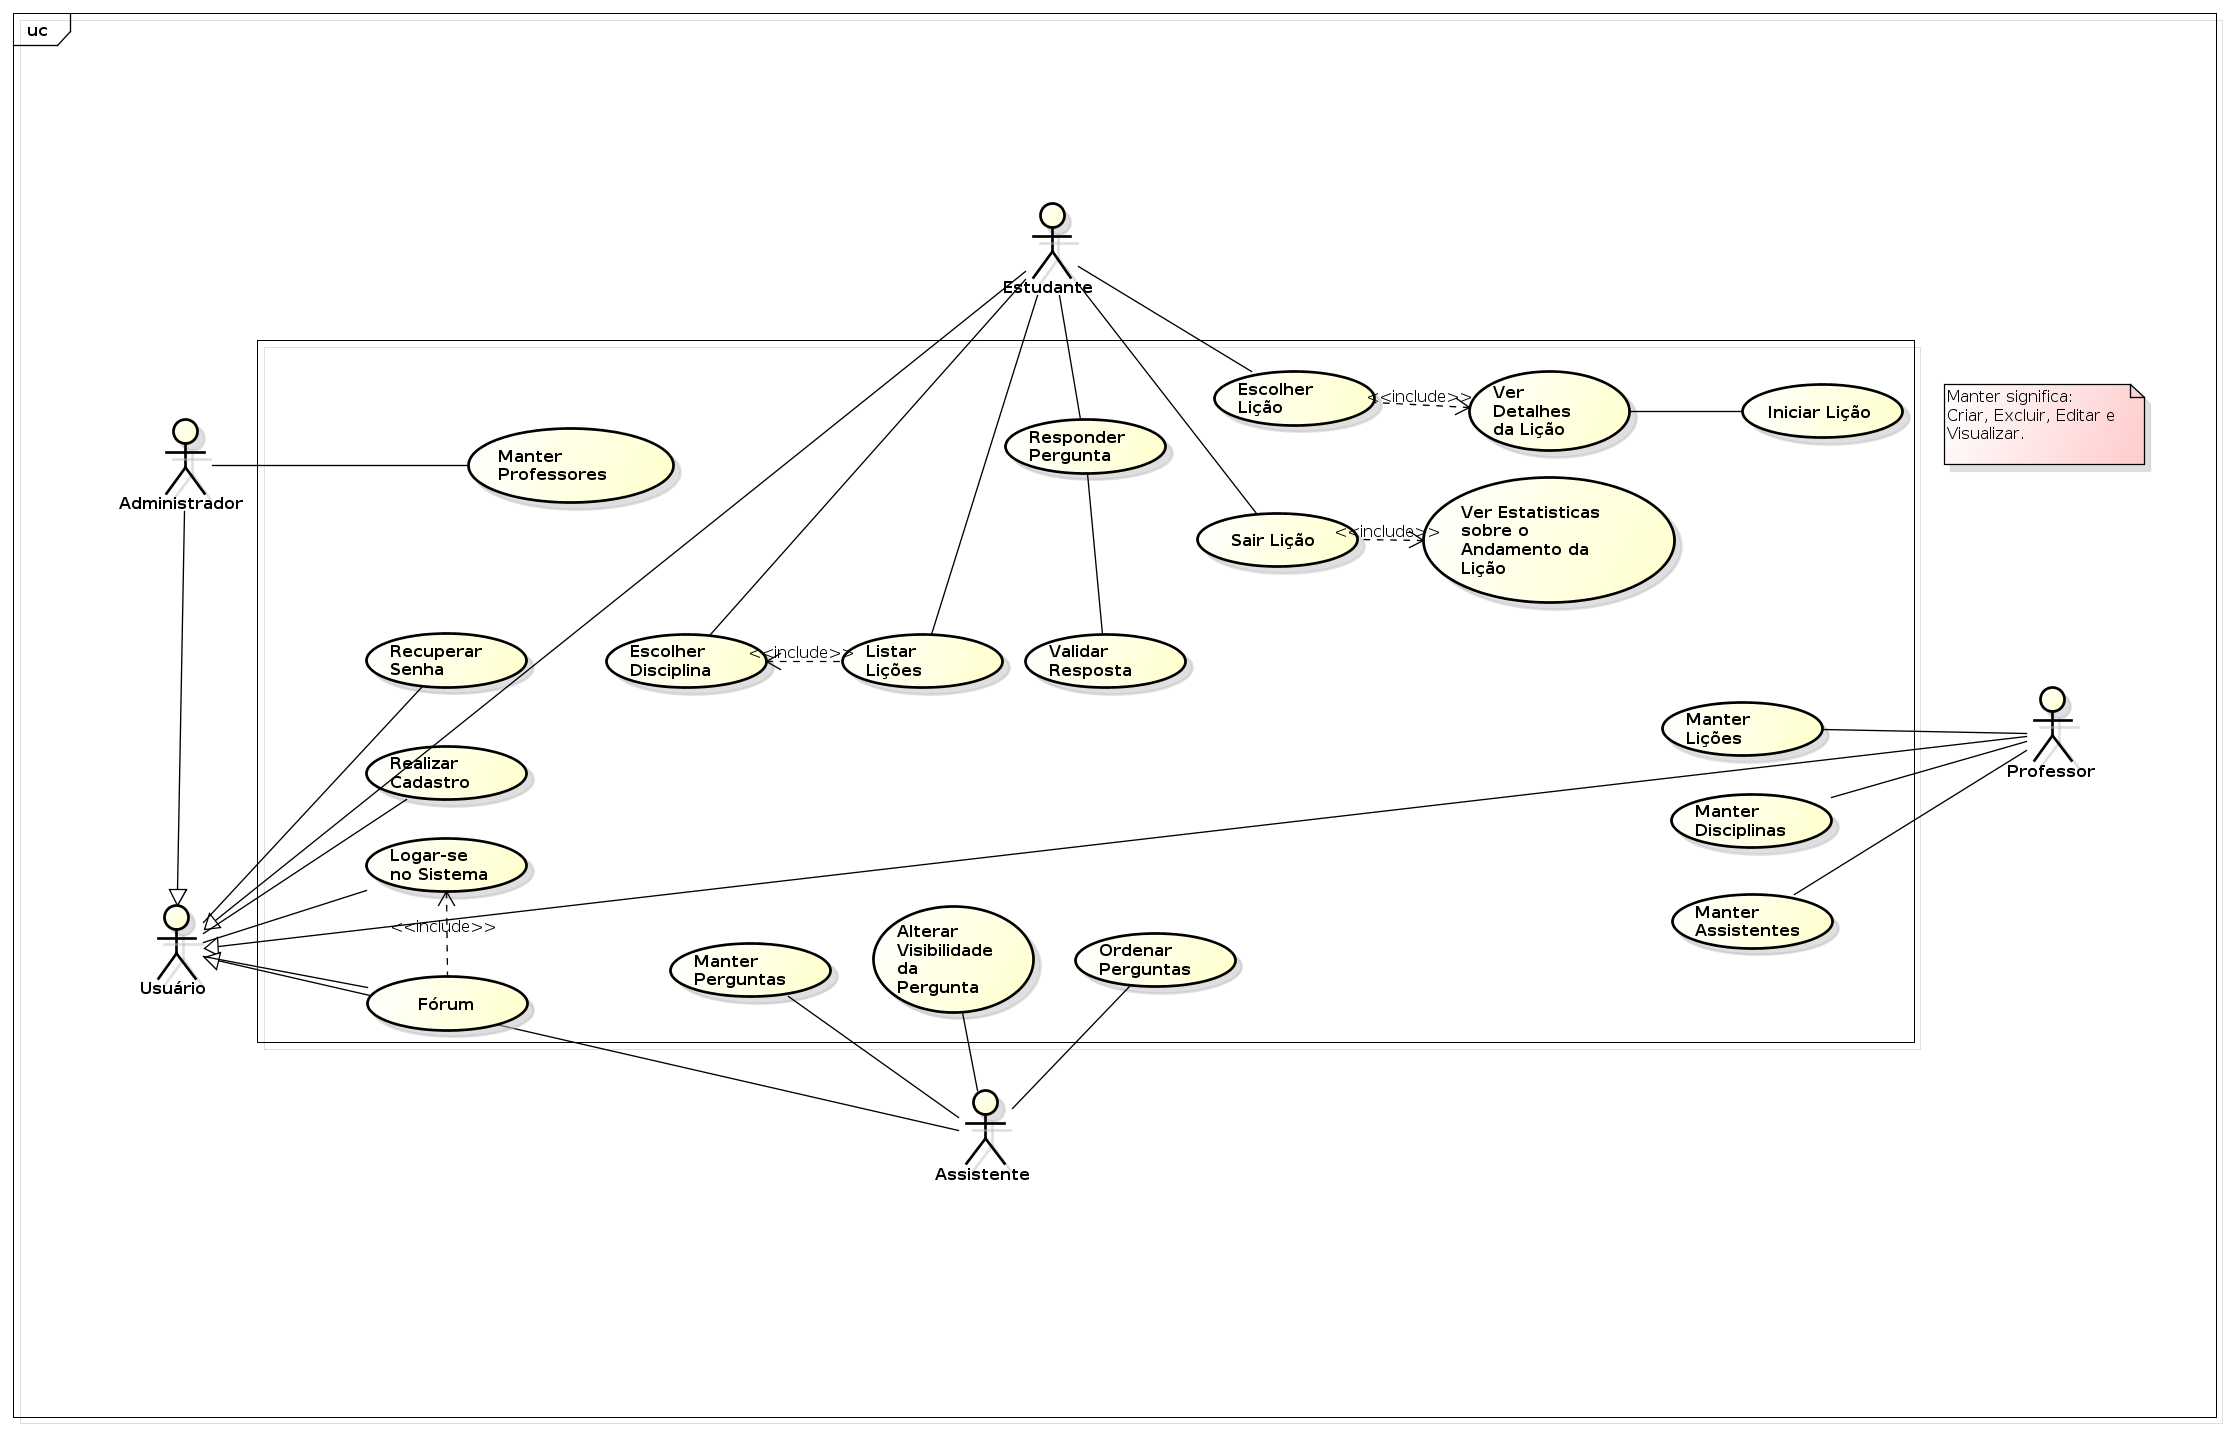
\includegraphics[width=18cm]{figuras/figura_casos_de_uso}
\label{figura_casos_de_uso}
\fnote{Fonte: Elaborado pelo autor}
\end{figure}

\subsection{Descri\c{c}\~ao dos Casos de Uso}

\begin{alineascomponto}
	\item Manter Professor: O Administrador terá uma opção onde poderá manter 
professores: isso funcionara da seguinte forma: Para cadastrar, o Administrador 
logado, gera um código de alguns caracteres e dar ao professor, o professor de 
posse desse código, entra na tela de cadastro dos usuário e escolhe o tipo de 
usuário que ele quer se cadastrar e informa o código de acesso que ele possui, 
assim ele terá permissão para se cadastrar como Professor.

	\item Manter Assistente: De forma análoga ao Administrador, o professor 
também irá gerar um código e entregar ao assistente, o assistente de posse 
desse código irá entrar na tela de cadastro do sistema, informar o tipo de 
usuário e o código de acesso.

	\item Recuperação de Senha: No momento do cadastro, cada usuário devera 
indicar um email v\'alido, caso futuramente o usuário necessite 
alterar a senha, um email será enviado à esse email cadastrado com um link onde 
o mesmo poder\'a acessar para recuperar a senha.

	\item Manter Conte\'udos: Apenas os professores terão permissão para manter 
conte\'udos e lições, ao adicionar uma lição, ele terá que informar apenas o 
nome da lição e ao adicionar uma lição, ele terá que informar os 
Pré-Requisitos(Outras lições que eles recomendam ter sido concluídas para se 
prosseguir na atual) e Sugestões de Estudo (outras lições que eles recomendam 
seguir após concluir essa lição) para aquela lição assim como a quantidade 
máxima de pulos que o aluno poderá realizar naquela lição.

	\item Manter Problemas: Cada lição possuirá uma lista de problemas e os 
mesmos serão adicionadas pelos assistentes. Quando um assistente adicionar 
um problema, ele terá de informar a qual lição que ele pertence, os itens que 
ela terá, assim como o item correto, a ajuda caso esse problema necessite ter, 
a quantidade de pontos que ele terá e se ele irá ficar visível imediatamente 
para os alunos ou não.

	\item Ver Detalhes da Lição: Quando o aluno optar por responder as perguntas 
de uma determinada lição, antes de mais nada, ele precisa saber os detalhes 
daquela lição, detalhes do tipo: Quantidade de questões, Máximo de Saltos 
Permitidos, Pré-Requisitos, Curiosidades sobre o conteúdo daquela lição.

	\item Sair da Lição: Enquanto o aluno estiver resolvendo os problemas, o 
sistema devera lhe oferecer a opção dele sair da lição, quando ele sair, ele 
terá de ver as estatísticas referentes ao andamento dele naquela lição como: 
Acertos, Erros, Saltos, Quantidade de Pontos Acumulados e também uma lista com 
as lições sugeridas.
	
	\item Ordenar Problemas: Quando o bolsista adicionar um problema, ela será 
adicionada automaticamente logo depois dos outros problemas daquela lição(se 
pensarmos numa lista), mas ele deverá ter uma opção onde apenas arrastando 
os problema de posição ele possa reordena-los, utilizando apenas o mouse.

\end{alineascomponto}